% !TEX encoding = UTF-8 Unicode
\documentclass[10pt]{standalone}\usepackage{tikz,graphicx}
\usepackage{fontspec}
\setmainfont{Arial}
\setsansfont{Arial}\begin{document}

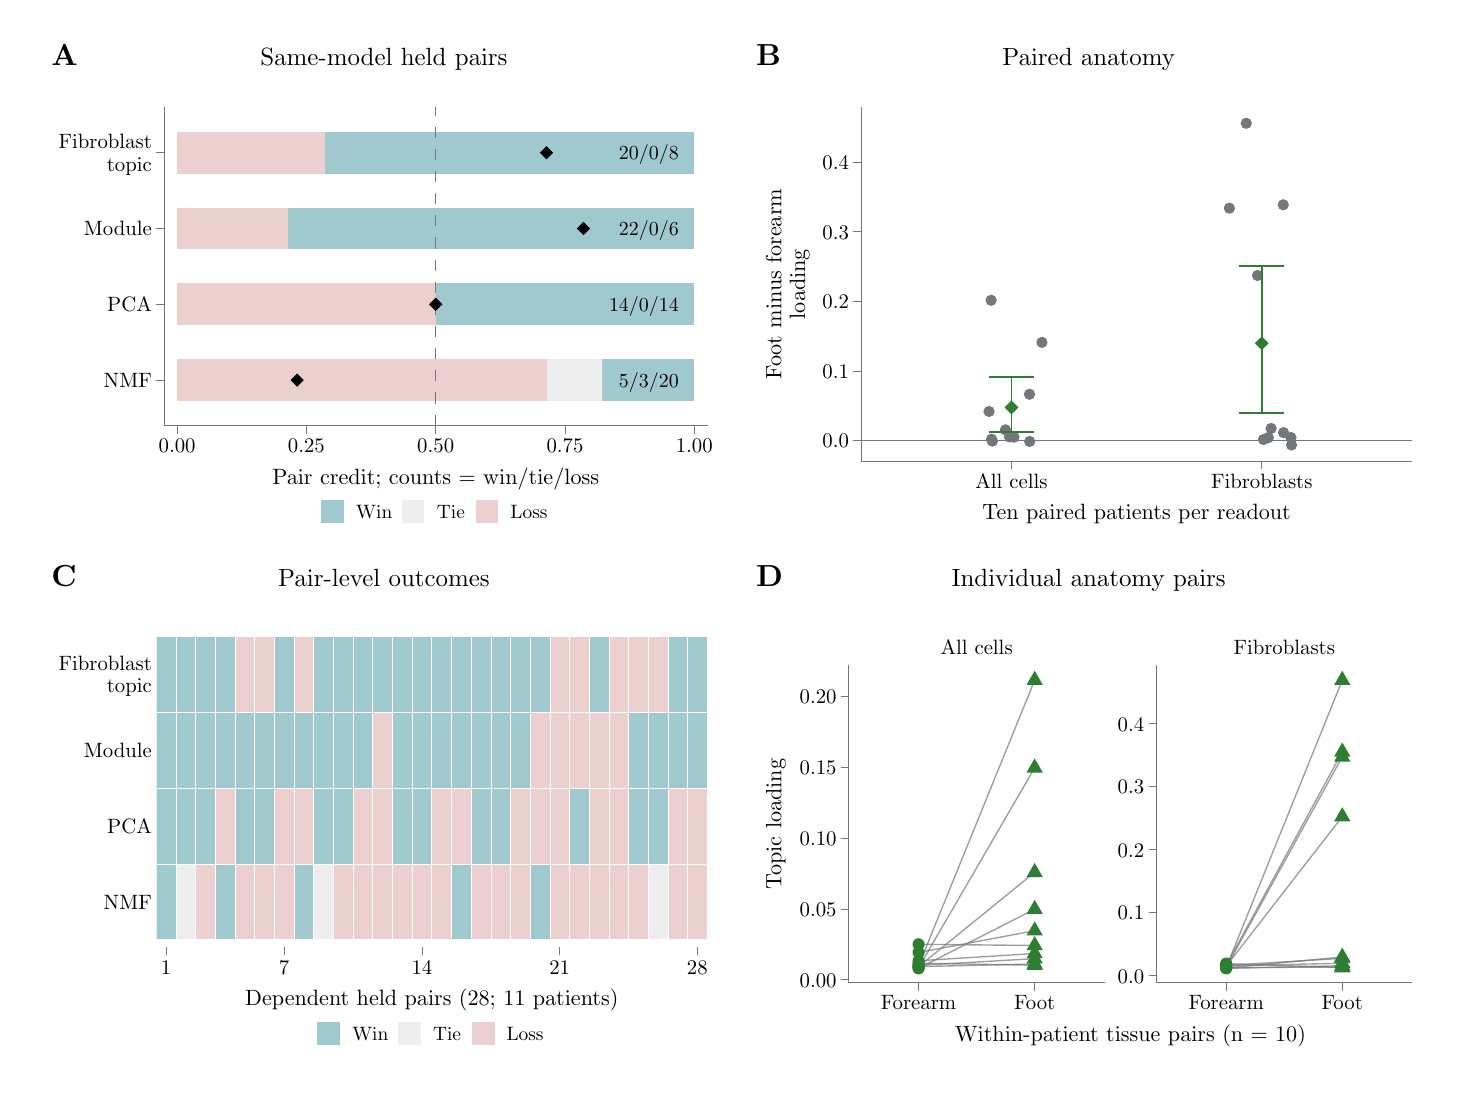
\begin{tikzpicture}[x=1pt,y=1pt]
\definecolor{fillColor}{RGB}{255,255,255}
\path[use as bounding box,fill=fillColor,fill opacity=0.00] (0,0) rectangle (512.15,375.58);
\begin{scope}
\path[clip] (  0.00,  0.00) rectangle (512.15,375.58);
\definecolor{drawColor}{RGB}{0,0,0}

\node[text=drawColor,anchor=base west,inner sep=0pt, outer sep=0pt, scale=  1.10] at (  8.54,362.01) {\bfseries A};

\node[text=drawColor,anchor=base,inner sep=0pt, outer sep=0pt, scale=  0.90] at (128.75,362.02) {Same-model held pairs};
\end{scope}
\begin{scope}
\path[clip] (  8.54,192.77) rectangle (248.96,351.96);
\definecolor{fillColor}{RGB}{255,255,255}

\path[fill=fillColor] (  8.54,192.77) rectangle (248.96,351.96);
\end{scope}
\begin{scope}
\path[clip] ( 49.33,231.77) rectangle (245.55,346.84);
\definecolor{fillColor}{RGB}{255,255,255}

\path[fill=fillColor] ( 49.33,231.77) rectangle (245.55,346.84);
\definecolor{fillColor}{RGB}{159,200,207}

\path[fill=fillColor] (107.39,322.87) rectangle (240.88,337.94);

\path[fill=fillColor] ( 94.04,295.47) rectangle (240.88,310.54);

\path[fill=fillColor] (147.44,268.07) rectangle (240.88,283.14);

\path[fill=fillColor] (207.50,240.68) rectangle (240.88,255.74);
\definecolor{fillColor}{RGB}{238,238,238}

\path[fill=fillColor] (107.39,322.87) rectangle (107.39,337.94);

\path[fill=fillColor] ( 94.04,295.47) rectangle ( 94.04,310.54);

\path[fill=fillColor] (147.44,268.07) rectangle (147.44,283.14);

\path[fill=fillColor] (187.48,240.68) rectangle (207.50,255.74);
\definecolor{fillColor}{RGB}{236,207,207}

\path[fill=fillColor] ( 54.00,322.87) rectangle (107.39,337.94);

\path[fill=fillColor] ( 54.00,295.47) rectangle ( 94.04,310.54);

\path[fill=fillColor] ( 54.00,268.07) rectangle (147.44,283.14);

\path[fill=fillColor] ( 54.00,240.68) rectangle (187.48,255.74);
\definecolor{drawColor}{RGB}{115,119,123}

\path[draw=drawColor,line width= 0.3pt,dash pattern=on 4pt off 4pt ,line join=round] (147.44,231.77) -- (147.44,346.84);
\definecolor{fillColor}{RGB}{0,0,0}

\path[fill=fillColor] (185.08,330.40) --
	(187.48,332.80) --
	(189.88,330.40) --
	(187.48,328.00) --
	cycle;

\path[fill=fillColor] (198.43,303.00) --
	(200.83,305.40) --
	(203.23,303.00) --
	(200.83,300.60) --
	cycle;

\path[fill=fillColor] (145.04,275.61) --
	(147.44,278.01) --
	(149.84,275.61) --
	(147.44,273.21) --
	cycle;

\path[fill=fillColor] ( 94.98,248.21) --
	( 97.38,250.61) --
	( 99.78,248.21) --
	( 97.38,245.81) --
	cycle;
\definecolor{drawColor}{RGB}{0,0,0}

\node[text=drawColor,anchor=base east,inner sep=0pt, outer sep=0pt, scale=  0.72] at (235.27,327.82) {20/0/8};

\node[text=drawColor,anchor=base east,inner sep=0pt, outer sep=0pt, scale=  0.72] at (235.27,300.43) {22/0/6};

\node[text=drawColor,anchor=base east,inner sep=0pt, outer sep=0pt, scale=  0.72] at (235.27,273.03) {14/0/14};

\node[text=drawColor,anchor=base east,inner sep=0pt, outer sep=0pt, scale=  0.72] at (235.27,245.63) {5/3/20};
\end{scope}
\begin{scope}
\path[clip] (  0.00,  0.00) rectangle (512.15,375.58);
\definecolor{drawColor}{RGB}{115,119,123}

\path[draw=drawColor,line width= 0.3pt,line join=round,line cap=rect] ( 49.33,231.77) --
	( 49.33,346.84);
\end{scope}
\begin{scope}
\path[clip] (  0.00,  0.00) rectangle (512.15,375.58);
\definecolor{drawColor}{RGB}{0,0,0}

\node[text=drawColor,anchor=base east,inner sep=0pt, outer sep=0pt, scale=  0.75] at ( 44.88,245.53) {NMF};

\node[text=drawColor,anchor=base east,inner sep=0pt, outer sep=0pt, scale=  0.75] at ( 44.88,272.92) {PCA};

\node[text=drawColor,anchor=base east,inner sep=0pt, outer sep=0pt, scale=  0.75] at ( 44.88,300.32) {Module};

\node[text=drawColor,anchor=base east,inner sep=0pt, outer sep=0pt, scale=  0.75] at ( 44.88,331.77) {Fibroblast};

\node[text=drawColor,anchor=base east,inner sep=0pt, outer sep=0pt, scale=  0.75] at ( 44.88,323.67) {topic};
\end{scope}
\begin{scope}
\path[clip] (  0.00,  0.00) rectangle (512.15,375.58);
\definecolor{drawColor}{RGB}{115,119,123}

\path[draw=drawColor,line width= 0.3pt,line join=round] ( 46.48,248.21) --
	( 49.33,248.21);

\path[draw=drawColor,line width= 0.3pt,line join=round] ( 46.48,275.61) --
	( 49.33,275.61);

\path[draw=drawColor,line width= 0.3pt,line join=round] ( 46.48,303.00) --
	( 49.33,303.00);

\path[draw=drawColor,line width= 0.3pt,line join=round] ( 46.48,330.40) --
	( 49.33,330.40);
\end{scope}
\begin{scope}
\path[clip] (  0.00,  0.00) rectangle (512.15,375.58);
\definecolor{drawColor}{RGB}{115,119,123}

\path[draw=drawColor,line width= 0.3pt,line join=round,line cap=rect] ( 49.33,231.77) --
	(245.55,231.77);
\end{scope}
\begin{scope}
\path[clip] (  0.00,  0.00) rectangle (512.15,375.58);
\definecolor{drawColor}{RGB}{115,119,123}

\path[draw=drawColor,line width= 0.3pt,line join=round] ( 54.00,228.93) --
	( 54.00,231.77);

\path[draw=drawColor,line width= 0.3pt,line join=round] (100.72,228.93) --
	(100.72,231.77);

\path[draw=drawColor,line width= 0.3pt,line join=round] (147.44,228.93) --
	(147.44,231.77);

\path[draw=drawColor,line width= 0.3pt,line join=round] (194.16,228.93) --
	(194.16,231.77);

\path[draw=drawColor,line width= 0.3pt,line join=round] (240.88,228.93) --
	(240.88,231.77);
\end{scope}
\begin{scope}
\path[clip] (  0.00,  0.00) rectangle (512.15,375.58);
\definecolor{drawColor}{RGB}{0,0,0}

\node[text=drawColor,anchor=base,inner sep=0pt, outer sep=0pt, scale=  0.75] at ( 54.00,221.96) {0.00};

\node[text=drawColor,anchor=base,inner sep=0pt, outer sep=0pt, scale=  0.75] at (100.72,221.96) {0.25};

\node[text=drawColor,anchor=base,inner sep=0pt, outer sep=0pt, scale=  0.75] at (147.44,221.96) {0.50};

\node[text=drawColor,anchor=base,inner sep=0pt, outer sep=0pt, scale=  0.75] at (194.16,221.96) {0.75};

\node[text=drawColor,anchor=base,inner sep=0pt, outer sep=0pt, scale=  0.75] at (240.88,221.96) {1.00};
\end{scope}
\begin{scope}
\path[clip] (  0.00,  0.00) rectangle (512.15,375.58);
\definecolor{drawColor}{RGB}{0,0,0}

\node[text=drawColor,anchor=base,inner sep=0pt, outer sep=0pt, scale=  0.80] at (147.44,210.67) {Pair credit; counts = win/tie/loss};
\end{scope}
\begin{scope}
\path[clip] (  0.00,  0.00) rectangle (512.15,375.58);
\definecolor{fillColor}{RGB}{255,255,255}

\path[fill=fillColor] (105.63,196.18) rectangle (189.25,205.29);
\end{scope}
\begin{scope}
\path[clip] (  0.00,  0.00) rectangle (512.15,375.58);
\definecolor{fillColor}{RGB}{255,255,255}

\path[fill=fillColor] (105.63,196.18) rectangle (114.73,205.29);
\definecolor{fillColor}{RGB}{159,200,207}

\path[fill=fillColor] (106.14,196.70) rectangle (114.21,204.77);
\end{scope}
\begin{scope}
\path[clip] (  0.00,  0.00) rectangle (512.15,375.58);
\definecolor{fillColor}{RGB}{255,255,255}

\path[fill=fillColor] (134.79,196.18) rectangle (143.89,205.29);
\definecolor{fillColor}{RGB}{238,238,238}

\path[fill=fillColor] (135.30,196.70) rectangle (143.37,204.77);
\end{scope}
\begin{scope}
\path[clip] (  0.00,  0.00) rectangle (512.15,375.58);
\definecolor{fillColor}{RGB}{255,255,255}

\path[fill=fillColor] (161.36,196.18) rectangle (170.46,205.29);
\definecolor{fillColor}{RGB}{236,207,207}

\path[fill=fillColor] (161.87,196.70) rectangle (169.94,204.77);
\end{scope}
\begin{scope}
\path[clip] (  0.00,  0.00) rectangle (512.15,375.58);
\definecolor{drawColor}{RGB}{0,0,0}

\node[text=drawColor,anchor=base west,inner sep=0pt, outer sep=0pt, scale=  0.70] at (118.73,198.23) {Win};
\end{scope}
\begin{scope}
\path[clip] (  0.00,  0.00) rectangle (512.15,375.58);
\definecolor{drawColor}{RGB}{0,0,0}

\node[text=drawColor,anchor=base west,inner sep=0pt, outer sep=0pt, scale=  0.70] at (147.89,198.23) {Tie};
\end{scope}
\begin{scope}
\path[clip] (  0.00,  0.00) rectangle (512.15,375.58);
\definecolor{drawColor}{RGB}{0,0,0}

\node[text=drawColor,anchor=base west,inner sep=0pt, outer sep=0pt, scale=  0.70] at (174.46,198.23) {Loss};
\end{scope}
\begin{scope}
\path[clip] (  0.00,  0.00) rectangle (512.15,375.58);
\definecolor{drawColor}{RGB}{0,0,0}

\node[text=drawColor,anchor=base west,inner sep=0pt, outer sep=0pt, scale=  1.10] at (263.19,362.01) {\bfseries B};

\node[text=drawColor,anchor=base,inner sep=0pt, outer sep=0pt, scale=  0.90] at (383.40,362.02) {Paired anatomy};
\end{scope}
\begin{scope}
\path[clip] (263.19,192.77) rectangle (503.61,351.96);
\definecolor{fillColor}{RGB}{255,255,255}

\path[fill=fillColor] (263.19,192.77) rectangle (503.61,351.96);
\end{scope}
\begin{scope}
\path[clip] (301.22,218.97) rectangle (500.20,346.84);
\definecolor{fillColor}{RGB}{255,255,255}

\path[fill=fillColor] (301.22,218.97) rectangle (500.20,346.84);
\definecolor{drawColor}{RGB}{115,119,123}

\path[draw=drawColor,line width= 0.3pt,line join=round] (301.22,226.40) -- (500.20,226.40);
\definecolor{fillColor}{RGB}{115,119,123}

\path[draw=drawColor,line width= 0.3pt,line join=round,line cap=round,fill=fillColor] (347.38,236.89) circle (  1.87);

\path[draw=drawColor,line width= 0.3pt,line join=round,line cap=round,fill=fillColor] (366.50,261.86) circle (  1.87);

\path[draw=drawColor,line width= 0.3pt,line join=round,line cap=round,fill=fillColor] (354.74,227.69) circle (  1.87);

\path[draw=drawColor,line width= 0.3pt,line join=round,line cap=round,fill=fillColor] (362.00,243.12) circle (  1.87);

\path[draw=drawColor,line width= 0.3pt,line join=round,line cap=round,fill=fillColor] (353.32,230.26) circle (  1.87);

\path[draw=drawColor,line width= 0.3pt,line join=round,line cap=round,fill=fillColor] (356.40,227.60) circle (  1.87);

\path[draw=drawColor,line width= 0.3pt,line join=round,line cap=round,fill=fillColor] (348.60,226.19) circle (  1.87);

\path[draw=drawColor,line width= 0.3pt,line join=round,line cap=round,fill=fillColor] (348.13,277.07) circle (  1.87);

\path[draw=drawColor,line width= 0.3pt,line join=round,line cap=round,fill=fillColor] (362.07,226.05) circle (  1.87);

\path[draw=drawColor,line width= 0.3pt,line join=round,line cap=round,fill=fillColor] (348.29,226.87) circle (  1.87);

\path[draw=drawColor,line width= 0.3pt,line join=round,line cap=round,fill=fillColor] (444.39,286.03) circle (  1.87);

\path[draw=drawColor,line width= 0.3pt,line join=round,line cap=round,fill=fillColor] (434.23,310.35) circle (  1.87);

\path[draw=drawColor,line width= 0.3pt,line join=round,line cap=round,fill=fillColor] (453.80,229.24) circle (  1.87);

\path[draw=drawColor,line width= 0.3pt,line join=round,line cap=round,fill=fillColor] (453.70,311.57) circle (  1.87);

\path[draw=drawColor,line width= 0.3pt,line join=round,line cap=round,fill=fillColor] (456.68,224.78) circle (  1.87);

\path[draw=drawColor,line width= 0.3pt,line join=round,line cap=round,fill=fillColor] (456.48,227.47) circle (  1.87);

\path[draw=drawColor,line width= 0.3pt,line join=round,line cap=round,fill=fillColor] (448.30,227.45) circle (  1.87);

\path[draw=drawColor,line width= 0.3pt,line join=round,line cap=round,fill=fillColor] (440.33,341.03) circle (  1.87);

\path[draw=drawColor,line width= 0.3pt,line join=round,line cap=round,fill=fillColor] (449.30,230.75) circle (  1.87);

\path[draw=drawColor,line width= 0.3pt,line join=round,line cap=round,fill=fillColor] (446.55,226.75) circle (  1.87);
\definecolor{drawColor}{RGB}{46,125,50}

\path[draw=drawColor,line width= 0.7pt,line join=round] (347.35,249.43) --
	(363.63,249.43);

\path[draw=drawColor,line width= 0.7pt,line join=round] (355.49,249.43) --
	(355.49,229.39);

\path[draw=drawColor,line width= 0.7pt,line join=round] (347.35,229.39) --
	(363.63,229.39);

\path[draw=drawColor,line width= 0.7pt,line join=round] (437.79,289.50) --
	(454.07,289.50);

\path[draw=drawColor,line width= 0.7pt,line join=round] (445.93,289.50) --
	(445.93,236.28);

\path[draw=drawColor,line width= 0.7pt,line join=round] (437.79,236.28) --
	(454.07,236.28);
\definecolor{fillColor}{RGB}{46,125,50}

\path[fill=fillColor] (352.98,238.36) --
	(355.49,240.87) --
	(358.00,238.36) --
	(355.49,235.85) --
	cycle;

\path[fill=fillColor] (443.43,261.54) --
	(445.93,264.05) --
	(448.44,261.54) --
	(445.93,259.03) --
	cycle;
\end{scope}
\begin{scope}
\path[clip] (  0.00,  0.00) rectangle (512.15,375.58);
\definecolor{drawColor}{RGB}{115,119,123}

\path[draw=drawColor,line width= 0.3pt,line join=round,line cap=rect] (301.22,218.97) --
	(301.22,346.84);
\end{scope}
\begin{scope}
\path[clip] (  0.00,  0.00) rectangle (512.15,375.58);
\definecolor{drawColor}{RGB}{0,0,0}

\node[text=drawColor,anchor=base east,inner sep=0pt, outer sep=0pt, scale=  0.75] at (296.78,223.72) {0.0};

\node[text=drawColor,anchor=base east,inner sep=0pt, outer sep=0pt, scale=  0.75] at (296.78,248.85) {0.1};

\node[text=drawColor,anchor=base east,inner sep=0pt, outer sep=0pt, scale=  0.75] at (296.78,273.98) {0.2};

\node[text=drawColor,anchor=base east,inner sep=0pt, outer sep=0pt, scale=  0.75] at (296.78,299.11) {0.3};

\node[text=drawColor,anchor=base east,inner sep=0pt, outer sep=0pt, scale=  0.75] at (296.78,324.24) {0.4};
\end{scope}
\begin{scope}
\path[clip] (  0.00,  0.00) rectangle (512.15,375.58);
\definecolor{drawColor}{RGB}{115,119,123}

\path[draw=drawColor,line width= 0.3pt,line join=round] (298.38,226.40) --
	(301.22,226.40);

\path[draw=drawColor,line width= 0.3pt,line join=round] (298.38,251.53) --
	(301.22,251.53);

\path[draw=drawColor,line width= 0.3pt,line join=round] (298.38,276.66) --
	(301.22,276.66);

\path[draw=drawColor,line width= 0.3pt,line join=round] (298.38,301.79) --
	(301.22,301.79);

\path[draw=drawColor,line width= 0.3pt,line join=round] (298.38,326.92) --
	(301.22,326.92);
\end{scope}
\begin{scope}
\path[clip] (  0.00,  0.00) rectangle (512.15,375.58);
\definecolor{drawColor}{RGB}{115,119,123}

\path[draw=drawColor,line width= 0.3pt,line join=round,line cap=rect] (301.22,218.97) --
	(500.20,218.97);
\end{scope}
\begin{scope}
\path[clip] (  0.00,  0.00) rectangle (512.15,375.58);
\definecolor{drawColor}{RGB}{115,119,123}

\path[draw=drawColor,line width= 0.3pt,line join=round] (355.49,216.12) --
	(355.49,218.97);

\path[draw=drawColor,line width= 0.3pt,line join=round] (445.93,216.12) --
	(445.93,218.97);
\end{scope}
\begin{scope}
\path[clip] (  0.00,  0.00) rectangle (512.15,375.58);
\definecolor{drawColor}{RGB}{0,0,0}

\node[text=drawColor,anchor=base,inner sep=0pt, outer sep=0pt, scale=  0.75] at (355.49,209.15) {All cells};

\node[text=drawColor,anchor=base,inner sep=0pt, outer sep=0pt, scale=  0.75] at (445.93,209.15) {Fibroblasts};
\end{scope}
\begin{scope}
\path[clip] (  0.00,  0.00) rectangle (512.15,375.58);
\definecolor{drawColor}{RGB}{0,0,0}

\node[text=drawColor,anchor=base,inner sep=0pt, outer sep=0pt, scale=  0.80] at (400.71,197.87) {Ten paired patients per readout};
\end{scope}
\begin{scope}
\path[clip] (  0.00,  0.00) rectangle (512.15,375.58);
\definecolor{drawColor}{RGB}{0,0,0}

\node[text=drawColor,rotate= 90.00,anchor=base,inner sep=0pt, outer sep=0pt, scale=  0.80] at (272.33,282.90) {Foot minus forearm};

\node[text=drawColor,rotate= 90.00,anchor=base,inner sep=0pt, outer sep=0pt, scale=  0.80] at (280.97,282.90) {loading};
\end{scope}
\begin{scope}
\path[clip] (  0.00,  0.00) rectangle (512.15,375.58);
\definecolor{drawColor}{RGB}{0,0,0}

\node[text=drawColor,anchor=base west,inner sep=0pt, outer sep=0pt, scale=  1.10] at (  8.54,173.51) {\bfseries C};

\node[text=drawColor,anchor=base,inner sep=0pt, outer sep=0pt, scale=  0.90] at (128.75,173.52) {Pair-level outcomes};
\end{scope}
\begin{scope}
\path[clip] (  8.54,  4.27) rectangle (248.96,163.46);
\definecolor{fillColor}{RGB}{255,255,255}

\path[fill=fillColor] (  8.54,  4.27) rectangle (248.96,163.46);
\end{scope}
\begin{scope}
\path[clip] ( 46.48, 43.27) rectangle (245.55,158.34);
\definecolor{fillColor}{RGB}{255,255,255}

\path[fill=fillColor] ( 46.48, 43.27) rectangle (245.55,158.34);
\definecolor{drawColor}{RGB}{255,255,255}
\definecolor{fillColor}{RGB}{159,200,207}

\path[draw=drawColor,line width= 0.2pt,fill=fillColor] ( 46.48,128.20) rectangle ( 53.59,155.60);

\path[draw=drawColor,line width= 0.2pt,fill=fillColor] ( 46.48,100.81) rectangle ( 53.59,128.20);

\path[draw=drawColor,line width= 0.2pt,fill=fillColor] ( 46.48, 73.41) rectangle ( 53.59,100.81);

\path[draw=drawColor,line width= 0.2pt,fill=fillColor] ( 46.48, 46.01) rectangle ( 53.59, 73.41);

\path[draw=drawColor,line width= 0.2pt,fill=fillColor] ( 53.59,128.20) rectangle ( 60.70,155.60);

\path[draw=drawColor,line width= 0.2pt,fill=fillColor] ( 53.59,100.81) rectangle ( 60.70,128.20);

\path[draw=drawColor,line width= 0.2pt,fill=fillColor] ( 53.59, 73.41) rectangle ( 60.70,100.81);
\definecolor{fillColor}{RGB}{238,238,238}

\path[draw=drawColor,line width= 0.2pt,fill=fillColor] ( 53.59, 46.01) rectangle ( 60.70, 73.41);
\definecolor{fillColor}{RGB}{159,200,207}

\path[draw=drawColor,line width= 0.2pt,fill=fillColor] ( 60.70,128.20) rectangle ( 67.81,155.60);

\path[draw=drawColor,line width= 0.2pt,fill=fillColor] ( 60.70,100.81) rectangle ( 67.81,128.20);

\path[draw=drawColor,line width= 0.2pt,fill=fillColor] ( 60.70, 73.41) rectangle ( 67.81,100.81);
\definecolor{fillColor}{RGB}{236,207,207}

\path[draw=drawColor,line width= 0.2pt,fill=fillColor] ( 60.70, 46.01) rectangle ( 67.81, 73.41);
\definecolor{fillColor}{RGB}{159,200,207}

\path[draw=drawColor,line width= 0.2pt,fill=fillColor] ( 67.81,128.20) rectangle ( 74.92,155.60);

\path[draw=drawColor,line width= 0.2pt,fill=fillColor] ( 67.81,100.81) rectangle ( 74.92,128.20);
\definecolor{fillColor}{RGB}{236,207,207}

\path[draw=drawColor,line width= 0.2pt,fill=fillColor] ( 67.81, 73.41) rectangle ( 74.92,100.81);
\definecolor{fillColor}{RGB}{159,200,207}

\path[draw=drawColor,line width= 0.2pt,fill=fillColor] ( 67.81, 46.01) rectangle ( 74.92, 73.41);
\definecolor{fillColor}{RGB}{236,207,207}

\path[draw=drawColor,line width= 0.2pt,fill=fillColor] ( 74.92,128.20) rectangle ( 82.03,155.60);
\definecolor{fillColor}{RGB}{159,200,207}

\path[draw=drawColor,line width= 0.2pt,fill=fillColor] ( 74.92,100.81) rectangle ( 82.03,128.20);

\path[draw=drawColor,line width= 0.2pt,fill=fillColor] ( 74.92, 73.41) rectangle ( 82.03,100.81);
\definecolor{fillColor}{RGB}{236,207,207}

\path[draw=drawColor,line width= 0.2pt,fill=fillColor] ( 74.92, 46.01) rectangle ( 82.03, 73.41);

\path[draw=drawColor,line width= 0.2pt,fill=fillColor] ( 82.03,128.20) rectangle ( 89.14,155.60);
\definecolor{fillColor}{RGB}{159,200,207}

\path[draw=drawColor,line width= 0.2pt,fill=fillColor] ( 82.03,100.81) rectangle ( 89.14,128.20);

\path[draw=drawColor,line width= 0.2pt,fill=fillColor] ( 82.03, 73.41) rectangle ( 89.14,100.81);
\definecolor{fillColor}{RGB}{236,207,207}

\path[draw=drawColor,line width= 0.2pt,fill=fillColor] ( 82.03, 46.01) rectangle ( 89.14, 73.41);
\definecolor{fillColor}{RGB}{159,200,207}

\path[draw=drawColor,line width= 0.2pt,fill=fillColor] ( 89.14,128.20) rectangle ( 96.25,155.60);

\path[draw=drawColor,line width= 0.2pt,fill=fillColor] ( 89.14,100.81) rectangle ( 96.25,128.20);
\definecolor{fillColor}{RGB}{236,207,207}

\path[draw=drawColor,line width= 0.2pt,fill=fillColor] ( 89.14, 73.41) rectangle ( 96.25,100.81);

\path[draw=drawColor,line width= 0.2pt,fill=fillColor] ( 89.14, 46.01) rectangle ( 96.25, 73.41);

\path[draw=drawColor,line width= 0.2pt,fill=fillColor] ( 96.25,128.20) rectangle (103.36,155.60);
\definecolor{fillColor}{RGB}{159,200,207}

\path[draw=drawColor,line width= 0.2pt,fill=fillColor] ( 96.25,100.81) rectangle (103.36,128.20);
\definecolor{fillColor}{RGB}{236,207,207}

\path[draw=drawColor,line width= 0.2pt,fill=fillColor] ( 96.25, 73.41) rectangle (103.36,100.81);
\definecolor{fillColor}{RGB}{159,200,207}

\path[draw=drawColor,line width= 0.2pt,fill=fillColor] ( 96.25, 46.01) rectangle (103.36, 73.41);

\path[draw=drawColor,line width= 0.2pt,fill=fillColor] (103.36,128.20) rectangle (110.47,155.60);

\path[draw=drawColor,line width= 0.2pt,fill=fillColor] (103.36,100.81) rectangle (110.47,128.20);

\path[draw=drawColor,line width= 0.2pt,fill=fillColor] (103.36, 73.41) rectangle (110.47,100.81);
\definecolor{fillColor}{RGB}{238,238,238}

\path[draw=drawColor,line width= 0.2pt,fill=fillColor] (103.36, 46.01) rectangle (110.47, 73.41);
\definecolor{fillColor}{RGB}{159,200,207}

\path[draw=drawColor,line width= 0.2pt,fill=fillColor] (110.47,128.20) rectangle (117.58,155.60);

\path[draw=drawColor,line width= 0.2pt,fill=fillColor] (110.47,100.81) rectangle (117.58,128.20);

\path[draw=drawColor,line width= 0.2pt,fill=fillColor] (110.47, 73.41) rectangle (117.58,100.81);
\definecolor{fillColor}{RGB}{236,207,207}

\path[draw=drawColor,line width= 0.2pt,fill=fillColor] (110.47, 46.01) rectangle (117.58, 73.41);
\definecolor{fillColor}{RGB}{159,200,207}

\path[draw=drawColor,line width= 0.2pt,fill=fillColor] (117.58,128.20) rectangle (124.68,155.60);

\path[draw=drawColor,line width= 0.2pt,fill=fillColor] (117.58,100.81) rectangle (124.68,128.20);
\definecolor{fillColor}{RGB}{236,207,207}

\path[draw=drawColor,line width= 0.2pt,fill=fillColor] (117.58, 73.41) rectangle (124.68,100.81);

\path[draw=drawColor,line width= 0.2pt,fill=fillColor] (117.58, 46.01) rectangle (124.68, 73.41);
\definecolor{fillColor}{RGB}{159,200,207}

\path[draw=drawColor,line width= 0.2pt,fill=fillColor] (124.68,128.20) rectangle (131.79,155.60);
\definecolor{fillColor}{RGB}{236,207,207}

\path[draw=drawColor,line width= 0.2pt,fill=fillColor] (124.68,100.81) rectangle (131.79,128.20);

\path[draw=drawColor,line width= 0.2pt,fill=fillColor] (124.68, 73.41) rectangle (131.79,100.81);

\path[draw=drawColor,line width= 0.2pt,fill=fillColor] (124.68, 46.01) rectangle (131.79, 73.41);
\definecolor{fillColor}{RGB}{159,200,207}

\path[draw=drawColor,line width= 0.2pt,fill=fillColor] (131.79,128.20) rectangle (138.90,155.60);

\path[draw=drawColor,line width= 0.2pt,fill=fillColor] (131.79,100.81) rectangle (138.90,128.20);

\path[draw=drawColor,line width= 0.2pt,fill=fillColor] (131.79, 73.41) rectangle (138.90,100.81);
\definecolor{fillColor}{RGB}{236,207,207}

\path[draw=drawColor,line width= 0.2pt,fill=fillColor] (131.79, 46.01) rectangle (138.90, 73.41);
\definecolor{fillColor}{RGB}{159,200,207}

\path[draw=drawColor,line width= 0.2pt,fill=fillColor] (138.90,128.20) rectangle (146.01,155.60);

\path[draw=drawColor,line width= 0.2pt,fill=fillColor] (138.90,100.81) rectangle (146.01,128.20);

\path[draw=drawColor,line width= 0.2pt,fill=fillColor] (138.90, 73.41) rectangle (146.01,100.81);
\definecolor{fillColor}{RGB}{236,207,207}

\path[draw=drawColor,line width= 0.2pt,fill=fillColor] (138.90, 46.01) rectangle (146.01, 73.41);
\definecolor{fillColor}{RGB}{159,200,207}

\path[draw=drawColor,line width= 0.2pt,fill=fillColor] (146.01,128.20) rectangle (153.12,155.60);

\path[draw=drawColor,line width= 0.2pt,fill=fillColor] (146.01,100.81) rectangle (153.12,128.20);
\definecolor{fillColor}{RGB}{236,207,207}

\path[draw=drawColor,line width= 0.2pt,fill=fillColor] (146.01, 73.41) rectangle (153.12,100.81);

\path[draw=drawColor,line width= 0.2pt,fill=fillColor] (146.01, 46.01) rectangle (153.12, 73.41);
\definecolor{fillColor}{RGB}{159,200,207}

\path[draw=drawColor,line width= 0.2pt,fill=fillColor] (153.12,128.20) rectangle (160.23,155.60);

\path[draw=drawColor,line width= 0.2pt,fill=fillColor] (153.12,100.81) rectangle (160.23,128.20);
\definecolor{fillColor}{RGB}{236,207,207}

\path[draw=drawColor,line width= 0.2pt,fill=fillColor] (153.12, 73.41) rectangle (160.23,100.81);
\definecolor{fillColor}{RGB}{159,200,207}

\path[draw=drawColor,line width= 0.2pt,fill=fillColor] (153.12, 46.01) rectangle (160.23, 73.41);

\path[draw=drawColor,line width= 0.2pt,fill=fillColor] (160.23,128.20) rectangle (167.34,155.60);

\path[draw=drawColor,line width= 0.2pt,fill=fillColor] (160.23,100.81) rectangle (167.34,128.20);

\path[draw=drawColor,line width= 0.2pt,fill=fillColor] (160.23, 73.41) rectangle (167.34,100.81);
\definecolor{fillColor}{RGB}{236,207,207}

\path[draw=drawColor,line width= 0.2pt,fill=fillColor] (160.23, 46.01) rectangle (167.34, 73.41);
\definecolor{fillColor}{RGB}{159,200,207}

\path[draw=drawColor,line width= 0.2pt,fill=fillColor] (167.34,128.20) rectangle (174.45,155.60);

\path[draw=drawColor,line width= 0.2pt,fill=fillColor] (167.34,100.81) rectangle (174.45,128.20);

\path[draw=drawColor,line width= 0.2pt,fill=fillColor] (167.34, 73.41) rectangle (174.45,100.81);
\definecolor{fillColor}{RGB}{236,207,207}

\path[draw=drawColor,line width= 0.2pt,fill=fillColor] (167.34, 46.01) rectangle (174.45, 73.41);
\definecolor{fillColor}{RGB}{159,200,207}

\path[draw=drawColor,line width= 0.2pt,fill=fillColor] (174.45,128.20) rectangle (181.56,155.60);

\path[draw=drawColor,line width= 0.2pt,fill=fillColor] (174.45,100.81) rectangle (181.56,128.20);
\definecolor{fillColor}{RGB}{236,207,207}

\path[draw=drawColor,line width= 0.2pt,fill=fillColor] (174.45, 73.41) rectangle (181.56,100.81);

\path[draw=drawColor,line width= 0.2pt,fill=fillColor] (174.45, 46.01) rectangle (181.56, 73.41);
\definecolor{fillColor}{RGB}{159,200,207}

\path[draw=drawColor,line width= 0.2pt,fill=fillColor] (181.56,128.20) rectangle (188.67,155.60);
\definecolor{fillColor}{RGB}{236,207,207}

\path[draw=drawColor,line width= 0.2pt,fill=fillColor] (181.56,100.81) rectangle (188.67,128.20);

\path[draw=drawColor,line width= 0.2pt,fill=fillColor] (181.56, 73.41) rectangle (188.67,100.81);
\definecolor{fillColor}{RGB}{159,200,207}

\path[draw=drawColor,line width= 0.2pt,fill=fillColor] (181.56, 46.01) rectangle (188.67, 73.41);
\definecolor{fillColor}{RGB}{236,207,207}

\path[draw=drawColor,line width= 0.2pt,fill=fillColor] (188.67,128.20) rectangle (195.78,155.60);

\path[draw=drawColor,line width= 0.2pt,fill=fillColor] (188.67,100.81) rectangle (195.78,128.20);

\path[draw=drawColor,line width= 0.2pt,fill=fillColor] (188.67, 73.41) rectangle (195.78,100.81);

\path[draw=drawColor,line width= 0.2pt,fill=fillColor] (188.67, 46.01) rectangle (195.78, 73.41);

\path[draw=drawColor,line width= 0.2pt,fill=fillColor] (195.78,128.20) rectangle (202.89,155.60);

\path[draw=drawColor,line width= 0.2pt,fill=fillColor] (195.78,100.81) rectangle (202.89,128.20);
\definecolor{fillColor}{RGB}{159,200,207}

\path[draw=drawColor,line width= 0.2pt,fill=fillColor] (195.78, 73.41) rectangle (202.89,100.81);
\definecolor{fillColor}{RGB}{236,207,207}

\path[draw=drawColor,line width= 0.2pt,fill=fillColor] (195.78, 46.01) rectangle (202.89, 73.41);
\definecolor{fillColor}{RGB}{159,200,207}

\path[draw=drawColor,line width= 0.2pt,fill=fillColor] (202.89,128.20) rectangle (210.00,155.60);
\definecolor{fillColor}{RGB}{236,207,207}

\path[draw=drawColor,line width= 0.2pt,fill=fillColor] (202.89,100.81) rectangle (210.00,128.20);

\path[draw=drawColor,line width= 0.2pt,fill=fillColor] (202.89, 73.41) rectangle (210.00,100.81);

\path[draw=drawColor,line width= 0.2pt,fill=fillColor] (202.89, 46.01) rectangle (210.00, 73.41);

\path[draw=drawColor,line width= 0.2pt,fill=fillColor] (210.00,128.20) rectangle (217.11,155.60);

\path[draw=drawColor,line width= 0.2pt,fill=fillColor] (210.00,100.81) rectangle (217.11,128.20);

\path[draw=drawColor,line width= 0.2pt,fill=fillColor] (210.00, 73.41) rectangle (217.11,100.81);

\path[draw=drawColor,line width= 0.2pt,fill=fillColor] (210.00, 46.01) rectangle (217.11, 73.41);

\path[draw=drawColor,line width= 0.2pt,fill=fillColor] (217.11,128.20) rectangle (224.22,155.60);
\definecolor{fillColor}{RGB}{159,200,207}

\path[draw=drawColor,line width= 0.2pt,fill=fillColor] (217.11,100.81) rectangle (224.22,128.20);

\path[draw=drawColor,line width= 0.2pt,fill=fillColor] (217.11, 73.41) rectangle (224.22,100.81);
\definecolor{fillColor}{RGB}{236,207,207}

\path[draw=drawColor,line width= 0.2pt,fill=fillColor] (217.11, 46.01) rectangle (224.22, 73.41);

\path[draw=drawColor,line width= 0.2pt,fill=fillColor] (224.22,128.20) rectangle (231.33,155.60);
\definecolor{fillColor}{RGB}{159,200,207}

\path[draw=drawColor,line width= 0.2pt,fill=fillColor] (224.22,100.81) rectangle (231.33,128.20);

\path[draw=drawColor,line width= 0.2pt,fill=fillColor] (224.22, 73.41) rectangle (231.33,100.81);
\definecolor{fillColor}{RGB}{238,238,238}

\path[draw=drawColor,line width= 0.2pt,fill=fillColor] (224.22, 46.01) rectangle (231.33, 73.41);
\definecolor{fillColor}{RGB}{159,200,207}

\path[draw=drawColor,line width= 0.2pt,fill=fillColor] (231.33,128.20) rectangle (238.44,155.60);

\path[draw=drawColor,line width= 0.2pt,fill=fillColor] (231.33,100.81) rectangle (238.44,128.20);
\definecolor{fillColor}{RGB}{236,207,207}

\path[draw=drawColor,line width= 0.2pt,fill=fillColor] (231.33, 73.41) rectangle (238.44,100.81);

\path[draw=drawColor,line width= 0.2pt,fill=fillColor] (231.33, 46.01) rectangle (238.44, 73.41);
\definecolor{fillColor}{RGB}{159,200,207}

\path[draw=drawColor,line width= 0.2pt,fill=fillColor] (238.44,128.20) rectangle (245.55,155.60);

\path[draw=drawColor,line width= 0.2pt,fill=fillColor] (238.44,100.81) rectangle (245.55,128.20);
\definecolor{fillColor}{RGB}{236,207,207}

\path[draw=drawColor,line width= 0.2pt,fill=fillColor] (238.44, 73.41) rectangle (245.55,100.81);

\path[draw=drawColor,line width= 0.2pt,fill=fillColor] (238.44, 46.01) rectangle (245.55, 73.41);
\end{scope}
\begin{scope}
\path[clip] (  0.00,  0.00) rectangle (512.15,375.58);
\definecolor{drawColor}{RGB}{0,0,0}

\node[text=drawColor,anchor=base east,inner sep=0pt, outer sep=0pt, scale=  0.75] at ( 44.88, 57.03) {NMF};

\node[text=drawColor,anchor=base east,inner sep=0pt, outer sep=0pt, scale=  0.75] at ( 44.88, 84.42) {PCA};

\node[text=drawColor,anchor=base east,inner sep=0pt, outer sep=0pt, scale=  0.75] at ( 44.88,111.82) {Module};

\node[text=drawColor,anchor=base east,inner sep=0pt, outer sep=0pt, scale=  0.75] at ( 44.88,143.27) {Fibroblast};

\node[text=drawColor,anchor=base east,inner sep=0pt, outer sep=0pt, scale=  0.75] at ( 44.88,135.17) {topic};
\end{scope}
\begin{scope}
\path[clip] (  0.00,  0.00) rectangle (512.15,375.58);
\definecolor{drawColor}{RGB}{115,119,123}

\path[draw=drawColor,line width= 0.3pt,line join=round] ( 50.03, 40.43) --
	( 50.03, 43.27);

\path[draw=drawColor,line width= 0.3pt,line join=round] ( 92.69, 40.43) --
	( 92.69, 43.27);

\path[draw=drawColor,line width= 0.3pt,line join=round] (142.46, 40.43) --
	(142.46, 43.27);

\path[draw=drawColor,line width= 0.3pt,line join=round] (192.23, 40.43) --
	(192.23, 43.27);

\path[draw=drawColor,line width= 0.3pt,line join=round] (241.99, 40.43) --
	(241.99, 43.27);
\end{scope}
\begin{scope}
\path[clip] (  0.00,  0.00) rectangle (512.15,375.58);
\definecolor{drawColor}{RGB}{0,0,0}

\node[text=drawColor,anchor=base,inner sep=0pt, outer sep=0pt, scale=  0.75] at ( 50.03, 33.46) {1};

\node[text=drawColor,anchor=base,inner sep=0pt, outer sep=0pt, scale=  0.75] at ( 92.69, 33.46) {7};

\node[text=drawColor,anchor=base,inner sep=0pt, outer sep=0pt, scale=  0.75] at (142.46, 33.46) {14};

\node[text=drawColor,anchor=base,inner sep=0pt, outer sep=0pt, scale=  0.75] at (192.23, 33.46) {21};

\node[text=drawColor,anchor=base,inner sep=0pt, outer sep=0pt, scale=  0.75] at (241.99, 33.46) {28};
\end{scope}
\begin{scope}
\path[clip] (  0.00,  0.00) rectangle (512.15,375.58);
\definecolor{drawColor}{RGB}{0,0,0}

\node[text=drawColor,anchor=base,inner sep=0pt, outer sep=0pt, scale=  0.80] at (146.01, 22.17) {Dependent held pairs (28; 11 patients)};
\end{scope}
\begin{scope}
\path[clip] (  0.00,  0.00) rectangle (512.15,375.58);
\definecolor{fillColor}{RGB}{255,255,255}

\path[fill=fillColor] (104.20,  7.68) rectangle (187.82, 16.79);
\end{scope}
\begin{scope}
\path[clip] (  0.00,  0.00) rectangle (512.15,375.58);
\definecolor{fillColor}{RGB}{255,255,255}

\path[fill=fillColor] (104.20,  7.68) rectangle (113.31, 16.79);
\definecolor{drawColor}{RGB}{255,255,255}
\definecolor{fillColor}{RGB}{159,200,207}

\path[draw=drawColor,line width= 0.2pt,fill=fillColor] (104.42,  7.90) rectangle (113.09, 16.57);
\end{scope}
\begin{scope}
\path[clip] (  0.00,  0.00) rectangle (512.15,375.58);
\definecolor{fillColor}{RGB}{255,255,255}

\path[fill=fillColor] (133.36,  7.68) rectangle (142.47, 16.79);
\definecolor{drawColor}{RGB}{255,255,255}
\definecolor{fillColor}{RGB}{238,238,238}

\path[draw=drawColor,line width= 0.2pt,fill=fillColor] (133.58,  7.90) rectangle (142.25, 16.57);
\end{scope}
\begin{scope}
\path[clip] (  0.00,  0.00) rectangle (512.15,375.58);
\definecolor{fillColor}{RGB}{255,255,255}

\path[fill=fillColor] (159.93,  7.68) rectangle (169.04, 16.79);
\definecolor{drawColor}{RGB}{255,255,255}
\definecolor{fillColor}{RGB}{236,207,207}

\path[draw=drawColor,line width= 0.2pt,fill=fillColor] (160.15,  7.90) rectangle (168.82, 16.57);
\end{scope}
\begin{scope}
\path[clip] (  0.00,  0.00) rectangle (512.15,375.58);
\definecolor{drawColor}{RGB}{0,0,0}

\node[text=drawColor,anchor=base west,inner sep=0pt, outer sep=0pt, scale=  0.70] at (117.31,  9.73) {Win};
\end{scope}
\begin{scope}
\path[clip] (  0.00,  0.00) rectangle (512.15,375.58);
\definecolor{drawColor}{RGB}{0,0,0}

\node[text=drawColor,anchor=base west,inner sep=0pt, outer sep=0pt, scale=  0.70] at (146.47,  9.73) {Tie};
\end{scope}
\begin{scope}
\path[clip] (  0.00,  0.00) rectangle (512.15,375.58);
\definecolor{drawColor}{RGB}{0,0,0}

\node[text=drawColor,anchor=base west,inner sep=0pt, outer sep=0pt, scale=  0.70] at (173.04,  9.73) {Loss};
\end{scope}
\begin{scope}
\path[clip] (  0.00,  0.00) rectangle (512.15,375.58);
\definecolor{drawColor}{RGB}{0,0,0}

\node[text=drawColor,anchor=base west,inner sep=0pt, outer sep=0pt, scale=  1.10] at (263.19,173.51) {\bfseries D};

\node[text=drawColor,anchor=base,inner sep=0pt, outer sep=0pt, scale=  0.90] at (383.40,173.52) {Individual anatomy pairs};
\end{scope}
\begin{scope}
\path[clip] (263.19,  4.27) rectangle (503.61,163.46);
\definecolor{fillColor}{RGB}{255,255,255}

\path[fill=fillColor] (263.19,  4.27) rectangle (503.61,163.46);
\end{scope}
\begin{scope}
\path[clip] (296.75, 30.47) rectangle (389.04,144.99);
\definecolor{fillColor}{RGB}{255,255,255}

\path[fill=fillColor] (296.75, 30.47) rectangle (389.04,144.99);
\definecolor{drawColor}{RGB}{115,119,123}

\path[draw=drawColor,draw opacity=0.70,line width= 0.5pt,line join=round] (321.92, 35.67) --
	(363.87, 57.03);

\path[draw=drawColor,draw opacity=0.70,line width= 0.5pt,line join=round] (321.92, 35.88) --
	(363.87,108.12);

\path[draw=drawColor,draw opacity=0.70,line width= 0.5pt,line join=round] (321.92, 38.41) --
	(363.87, 41.02);

\path[draw=drawColor,draw opacity=0.70,line width= 0.5pt,line join=round] (321.92, 36.28) --
	(363.87, 70.35);

\path[draw=drawColor,draw opacity=0.70,line width= 0.5pt,line join=round] (321.92, 41.40) --
	(363.87, 49.26);

\path[draw=drawColor,draw opacity=0.70,line width= 0.5pt,line join=round] (321.92, 36.74) --
	(363.87, 39.17);

\path[draw=drawColor,draw opacity=0.70,line width= 0.5pt,line join=round] (321.92, 44.36) --
	(363.87, 43.93);

\path[draw=drawColor,draw opacity=0.70,line width= 0.5pt,line join=round] (321.92, 36.57) --
	(363.87,139.79);

\path[draw=drawColor,draw opacity=0.70,line width= 0.5pt,line join=round] (321.92, 37.52) --
	(363.87, 36.80);

\path[draw=drawColor,draw opacity=0.70,line width= 0.5pt,line join=round] (321.92, 36.30) --
	(363.87, 37.24);
\definecolor{fillColor}{RGB}{46,125,50}

\path[fill=fillColor] (321.92, 35.67) circle (  2.19);

\path[fill=fillColor] (321.92, 35.88) circle (  2.19);

\path[fill=fillColor] (321.92, 38.41) circle (  2.19);

\path[fill=fillColor] (321.92, 36.28) circle (  2.19);

\path[fill=fillColor] (321.92, 41.40) circle (  2.19);

\path[fill=fillColor] (321.92, 36.74) circle (  2.19);

\path[fill=fillColor] (321.92, 44.36) circle (  2.19);

\path[fill=fillColor] (321.92, 36.57) circle (  2.19);

\path[fill=fillColor] (321.92, 37.52) circle (  2.19);

\path[fill=fillColor] (321.92, 36.30) circle (  2.19);

\path[fill=fillColor] (363.87, 60.43) --
	(366.82, 55.33) --
	(360.93, 55.33) --
	cycle;

\path[fill=fillColor] (363.87,111.52) --
	(366.82,106.42) --
	(360.93,106.42) --
	cycle;

\path[fill=fillColor] (363.87, 44.42) --
	(366.82, 39.32) --
	(360.93, 39.32) --
	cycle;

\path[fill=fillColor] (363.87, 73.75) --
	(366.82, 68.65) --
	(360.93, 68.65) --
	cycle;

\path[fill=fillColor] (363.87, 52.66) --
	(366.82, 47.56) --
	(360.93, 47.56) --
	cycle;

\path[fill=fillColor] (363.87, 42.57) --
	(366.82, 37.47) --
	(360.93, 37.47) --
	cycle;

\path[fill=fillColor] (363.87, 47.33) --
	(366.82, 42.23) --
	(360.93, 42.23) --
	cycle;

\path[fill=fillColor] (363.87,143.19) --
	(366.82,138.09) --
	(360.93,138.09) --
	cycle;

\path[fill=fillColor] (363.87, 40.20) --
	(366.82, 35.10) --
	(360.93, 35.10) --
	cycle;

\path[fill=fillColor] (363.87, 40.64) --
	(366.82, 35.54) --
	(360.93, 35.54) --
	cycle;
\end{scope}
\begin{scope}
\path[clip] (407.91, 30.47) rectangle (500.20,144.99);
\definecolor{fillColor}{RGB}{255,255,255}

\path[fill=fillColor] (407.91, 30.47) rectangle (500.20,144.99);
\definecolor{drawColor}{RGB}{115,119,123}

\path[draw=drawColor,draw opacity=0.70,line width= 0.5pt,line join=round] (433.08, 36.49) --
	(475.03, 90.51);

\path[draw=drawColor,draw opacity=0.70,line width= 0.5pt,line join=round] (433.08, 36.05) --
	(475.03,112.11);

\path[draw=drawColor,draw opacity=0.70,line width= 0.5pt,line join=round] (433.08, 36.72) --
	(475.03, 39.29);

\path[draw=drawColor,draw opacity=0.70,line width= 0.5pt,line join=round] (433.08, 36.73) --
	(475.03,113.89);

\path[draw=drawColor,draw opacity=0.70,line width= 0.5pt,line join=round] (433.08, 37.39) --
	(475.03, 35.92);

\path[draw=drawColor,draw opacity=0.70,line width= 0.5pt,line join=round] (433.08, 36.55) --
	(475.03, 37.51);

\path[draw=drawColor,draw opacity=0.70,line width= 0.5pt,line join=round] (433.08, 35.67) --
	(475.03, 36.62);

\path[draw=drawColor,draw opacity=0.70,line width= 0.5pt,line join=round] (433.08, 35.95) --
	(475.03,139.79);

\path[draw=drawColor,draw opacity=0.70,line width= 0.5pt,line join=round] (433.08, 35.82) --
	(475.03, 39.76);

\path[draw=drawColor,draw opacity=0.70,line width= 0.5pt,line join=round] (433.08, 35.87) --
	(475.03, 36.19);
\definecolor{fillColor}{RGB}{46,125,50}

\path[fill=fillColor] (433.08, 36.49) circle (  2.19);

\path[fill=fillColor] (433.08, 36.05) circle (  2.19);

\path[fill=fillColor] (433.08, 36.72) circle (  2.19);

\path[fill=fillColor] (433.08, 36.73) circle (  2.19);

\path[fill=fillColor] (433.08, 37.39) circle (  2.19);

\path[fill=fillColor] (433.08, 36.55) circle (  2.19);

\path[fill=fillColor] (433.08, 35.67) circle (  2.19);

\path[fill=fillColor] (433.08, 35.95) circle (  2.19);

\path[fill=fillColor] (433.08, 35.82) circle (  2.19);

\path[fill=fillColor] (433.08, 35.87) circle (  2.19);

\path[fill=fillColor] (475.03, 93.91) --
	(477.97, 88.81) --
	(472.09, 88.81) --
	cycle;

\path[fill=fillColor] (475.03,115.51) --
	(477.97,110.41) --
	(472.09,110.41) --
	cycle;

\path[fill=fillColor] (475.03, 42.69) --
	(477.97, 37.59) --
	(472.09, 37.59) --
	cycle;

\path[fill=fillColor] (475.03,117.29) --
	(477.97,112.19) --
	(472.09,112.19) --
	cycle;

\path[fill=fillColor] (475.03, 39.32) --
	(477.97, 34.22) --
	(472.09, 34.22) --
	cycle;

\path[fill=fillColor] (475.03, 40.91) --
	(477.97, 35.81) --
	(472.09, 35.81) --
	cycle;

\path[fill=fillColor] (475.03, 40.02) --
	(477.97, 34.92) --
	(472.09, 34.92) --
	cycle;

\path[fill=fillColor] (475.03,143.19) --
	(477.97,138.09) --
	(472.09,138.09) --
	cycle;

\path[fill=fillColor] (475.03, 43.16) --
	(477.97, 38.06) --
	(472.09, 38.06) --
	cycle;

\path[fill=fillColor] (475.03, 39.59) --
	(477.97, 34.49) --
	(472.09, 34.49) --
	cycle;
\end{scope}
\begin{scope}
\path[clip] (296.75,144.99) rectangle (389.04,158.34);
\definecolor{drawColor}{RGB}{0,0,0}

\node[text=drawColor,anchor=base,inner sep=0pt, outer sep=0pt, scale=  0.75] at (342.90,148.98) {All cells};
\end{scope}
\begin{scope}
\path[clip] (407.91,144.99) rectangle (500.20,158.34);
\definecolor{drawColor}{RGB}{0,0,0}

\node[text=drawColor,anchor=base,inner sep=0pt, outer sep=0pt, scale=  0.75] at (454.06,148.98) {Fibroblasts};
\end{scope}
\begin{scope}
\path[clip] (  0.00,  0.00) rectangle (512.15,375.58);
\definecolor{drawColor}{RGB}{115,119,123}

\path[draw=drawColor,line width= 0.3pt,line join=round,line cap=rect] (296.75, 30.47) --
	(389.04, 30.47);
\end{scope}
\begin{scope}
\path[clip] (  0.00,  0.00) rectangle (512.15,375.58);
\definecolor{drawColor}{RGB}{115,119,123}

\path[draw=drawColor,line width= 0.3pt,line join=round] (321.92, 27.62) --
	(321.92, 30.47);

\path[draw=drawColor,line width= 0.3pt,line join=round] (363.87, 27.62) --
	(363.87, 30.47);
\end{scope}
\begin{scope}
\path[clip] (  0.00,  0.00) rectangle (512.15,375.58);
\definecolor{drawColor}{RGB}{0,0,0}

\node[text=drawColor,anchor=base,inner sep=0pt, outer sep=0pt, scale=  0.75] at (321.92, 20.65) {Forearm};

\node[text=drawColor,anchor=base,inner sep=0pt, outer sep=0pt, scale=  0.75] at (363.87, 20.65) {Foot};
\end{scope}
\begin{scope}
\path[clip] (  0.00,  0.00) rectangle (512.15,375.58);
\definecolor{drawColor}{RGB}{115,119,123}

\path[draw=drawColor,line width= 0.3pt,line join=round,line cap=rect] (407.91, 30.47) --
	(500.20, 30.47);
\end{scope}
\begin{scope}
\path[clip] (  0.00,  0.00) rectangle (512.15,375.58);
\definecolor{drawColor}{RGB}{115,119,123}

\path[draw=drawColor,line width= 0.3pt,line join=round] (433.08, 27.62) --
	(433.08, 30.47);

\path[draw=drawColor,line width= 0.3pt,line join=round] (475.03, 27.62) --
	(475.03, 30.47);
\end{scope}
\begin{scope}
\path[clip] (  0.00,  0.00) rectangle (512.15,375.58);
\definecolor{drawColor}{RGB}{0,0,0}

\node[text=drawColor,anchor=base,inner sep=0pt, outer sep=0pt, scale=  0.75] at (433.08, 20.65) {Forearm};

\node[text=drawColor,anchor=base,inner sep=0pt, outer sep=0pt, scale=  0.75] at (475.03, 20.65) {Foot};
\end{scope}
\begin{scope}
\path[clip] (  0.00,  0.00) rectangle (512.15,375.58);
\definecolor{drawColor}{RGB}{115,119,123}

\path[draw=drawColor,line width= 0.3pt,line join=round,line cap=rect] (407.91, 30.47) --
	(407.91,144.99);
\end{scope}
\begin{scope}
\path[clip] (  0.00,  0.00) rectangle (512.15,375.58);
\definecolor{drawColor}{RGB}{0,0,0}

\node[text=drawColor,anchor=base east,inner sep=0pt, outer sep=0pt, scale=  0.75] at (403.47, 30.37) {0.0};

\node[text=drawColor,anchor=base east,inner sep=0pt, outer sep=0pt, scale=  0.75] at (403.47, 53.14) {0.1};

\node[text=drawColor,anchor=base east,inner sep=0pt, outer sep=0pt, scale=  0.75] at (403.47, 75.90) {0.2};

\node[text=drawColor,anchor=base east,inner sep=0pt, outer sep=0pt, scale=  0.75] at (403.47, 98.67) {0.3};

\node[text=drawColor,anchor=base east,inner sep=0pt, outer sep=0pt, scale=  0.75] at (403.47,121.43) {0.4};
\end{scope}
\begin{scope}
\path[clip] (  0.00,  0.00) rectangle (512.15,375.58);
\definecolor{drawColor}{RGB}{115,119,123}

\path[draw=drawColor,line width= 0.3pt,line join=round] (405.07, 33.06) --
	(407.91, 33.06);

\path[draw=drawColor,line width= 0.3pt,line join=round] (405.07, 55.82) --
	(407.91, 55.82);

\path[draw=drawColor,line width= 0.3pt,line join=round] (405.07, 78.59) --
	(407.91, 78.59);

\path[draw=drawColor,line width= 0.3pt,line join=round] (405.07,101.35) --
	(407.91,101.35);

\path[draw=drawColor,line width= 0.3pt,line join=round] (405.07,124.12) --
	(407.91,124.12);
\end{scope}
\begin{scope}
\path[clip] (  0.00,  0.00) rectangle (512.15,375.58);
\definecolor{drawColor}{RGB}{115,119,123}

\path[draw=drawColor,line width= 0.3pt,line join=round,line cap=rect] (296.75, 30.47) --
	(296.75,144.99);
\end{scope}
\begin{scope}
\path[clip] (  0.00,  0.00) rectangle (512.15,375.58);
\definecolor{drawColor}{RGB}{0,0,0}

\node[text=drawColor,anchor=base east,inner sep=0pt, outer sep=0pt, scale=  0.75] at (292.31, 28.86) {0.00};

\node[text=drawColor,anchor=base east,inner sep=0pt, outer sep=0pt, scale=  0.75] at (292.31, 54.46) {0.05};

\node[text=drawColor,anchor=base east,inner sep=0pt, outer sep=0pt, scale=  0.75] at (292.31, 80.05) {0.10};

\node[text=drawColor,anchor=base east,inner sep=0pt, outer sep=0pt, scale=  0.75] at (292.31,105.65) {0.15};

\node[text=drawColor,anchor=base east,inner sep=0pt, outer sep=0pt, scale=  0.75] at (292.31,131.25) {0.20};
\end{scope}
\begin{scope}
\path[clip] (  0.00,  0.00) rectangle (512.15,375.58);
\definecolor{drawColor}{RGB}{115,119,123}

\path[draw=drawColor,line width= 0.3pt,line join=round] (293.91, 31.54) --
	(296.75, 31.54);

\path[draw=drawColor,line width= 0.3pt,line join=round] (293.91, 57.14) --
	(296.75, 57.14);

\path[draw=drawColor,line width= 0.3pt,line join=round] (293.91, 82.74) --
	(296.75, 82.74);

\path[draw=drawColor,line width= 0.3pt,line join=round] (293.91,108.34) --
	(296.75,108.34);

\path[draw=drawColor,line width= 0.3pt,line join=round] (293.91,133.93) --
	(296.75,133.93);
\end{scope}
\begin{scope}
\path[clip] (  0.00,  0.00) rectangle (512.15,375.58);
\definecolor{drawColor}{RGB}{0,0,0}

\node[text=drawColor,anchor=base,inner sep=0pt, outer sep=0pt, scale=  0.80] at (398.48,  9.37) {Within-patient tissue pairs (n = 10)};
\end{scope}
\begin{scope}
\path[clip] (  0.00,  0.00) rectangle (512.15,375.58);
\definecolor{drawColor}{RGB}{0,0,0}

\node[text=drawColor,rotate= 90.00,anchor=base,inner sep=0pt, outer sep=0pt, scale=  0.80] at (272.33, 87.73) {Topic loading};
\end{scope}
\end{tikzpicture}

\end{document}
